\documentclass[]{article}
\usepackage{lmodern}
\usepackage{amssymb,amsmath}
\usepackage{ifxetex,ifluatex}
\usepackage{fixltx2e} % provides \textsubscript
\ifnum 0\ifxetex 1\fi\ifluatex 1\fi=0 % if pdftex
  \usepackage[T1]{fontenc}
  \usepackage[utf8]{inputenc}
\else % if luatex or xelatex
  \ifxetex
    \usepackage{mathspec}
  \else
    \usepackage{fontspec}
  \fi
  \defaultfontfeatures{Ligatures=TeX,Scale=MatchLowercase}
\fi
% use upquote if available, for straight quotes in verbatim environments
\IfFileExists{upquote.sty}{\usepackage{upquote}}{}
% use microtype if available
\IfFileExists{microtype.sty}{%
\usepackage{microtype}
\UseMicrotypeSet[protrusion]{basicmath} % disable protrusion for tt fonts
}{}
\usepackage[margin=1in]{geometry}
\usepackage{hyperref}
\hypersetup{unicode=true,
            pdftitle={NZ Generation History},
            pdfauthor={Ben Anderson (b.anderson@soton.ac.uk @dataknut)},
            pdfborder={0 0 0},
            breaklinks=true}
\urlstyle{same}  % don't use monospace font for urls
\usepackage{color}
\usepackage{fancyvrb}
\newcommand{\VerbBar}{|}
\newcommand{\VERB}{\Verb[commandchars=\\\{\}]}
\DefineVerbatimEnvironment{Highlighting}{Verbatim}{commandchars=\\\{\}}
% Add ',fontsize=\small' for more characters per line
\usepackage{framed}
\definecolor{shadecolor}{RGB}{248,248,248}
\newenvironment{Shaded}{\begin{snugshade}}{\end{snugshade}}
\newcommand{\KeywordTok}[1]{\textcolor[rgb]{0.13,0.29,0.53}{\textbf{#1}}}
\newcommand{\DataTypeTok}[1]{\textcolor[rgb]{0.13,0.29,0.53}{#1}}
\newcommand{\DecValTok}[1]{\textcolor[rgb]{0.00,0.00,0.81}{#1}}
\newcommand{\BaseNTok}[1]{\textcolor[rgb]{0.00,0.00,0.81}{#1}}
\newcommand{\FloatTok}[1]{\textcolor[rgb]{0.00,0.00,0.81}{#1}}
\newcommand{\ConstantTok}[1]{\textcolor[rgb]{0.00,0.00,0.00}{#1}}
\newcommand{\CharTok}[1]{\textcolor[rgb]{0.31,0.60,0.02}{#1}}
\newcommand{\SpecialCharTok}[1]{\textcolor[rgb]{0.00,0.00,0.00}{#1}}
\newcommand{\StringTok}[1]{\textcolor[rgb]{0.31,0.60,0.02}{#1}}
\newcommand{\VerbatimStringTok}[1]{\textcolor[rgb]{0.31,0.60,0.02}{#1}}
\newcommand{\SpecialStringTok}[1]{\textcolor[rgb]{0.31,0.60,0.02}{#1}}
\newcommand{\ImportTok}[1]{#1}
\newcommand{\CommentTok}[1]{\textcolor[rgb]{0.56,0.35,0.01}{\textit{#1}}}
\newcommand{\DocumentationTok}[1]{\textcolor[rgb]{0.56,0.35,0.01}{\textbf{\textit{#1}}}}
\newcommand{\AnnotationTok}[1]{\textcolor[rgb]{0.56,0.35,0.01}{\textbf{\textit{#1}}}}
\newcommand{\CommentVarTok}[1]{\textcolor[rgb]{0.56,0.35,0.01}{\textbf{\textit{#1}}}}
\newcommand{\OtherTok}[1]{\textcolor[rgb]{0.56,0.35,0.01}{#1}}
\newcommand{\FunctionTok}[1]{\textcolor[rgb]{0.00,0.00,0.00}{#1}}
\newcommand{\VariableTok}[1]{\textcolor[rgb]{0.00,0.00,0.00}{#1}}
\newcommand{\ControlFlowTok}[1]{\textcolor[rgb]{0.13,0.29,0.53}{\textbf{#1}}}
\newcommand{\OperatorTok}[1]{\textcolor[rgb]{0.81,0.36,0.00}{\textbf{#1}}}
\newcommand{\BuiltInTok}[1]{#1}
\newcommand{\ExtensionTok}[1]{#1}
\newcommand{\PreprocessorTok}[1]{\textcolor[rgb]{0.56,0.35,0.01}{\textit{#1}}}
\newcommand{\AttributeTok}[1]{\textcolor[rgb]{0.77,0.63,0.00}{#1}}
\newcommand{\RegionMarkerTok}[1]{#1}
\newcommand{\InformationTok}[1]{\textcolor[rgb]{0.56,0.35,0.01}{\textbf{\textit{#1}}}}
\newcommand{\WarningTok}[1]{\textcolor[rgb]{0.56,0.35,0.01}{\textbf{\textit{#1}}}}
\newcommand{\AlertTok}[1]{\textcolor[rgb]{0.94,0.16,0.16}{#1}}
\newcommand{\ErrorTok}[1]{\textcolor[rgb]{0.64,0.00,0.00}{\textbf{#1}}}
\newcommand{\NormalTok}[1]{#1}
\usepackage{graphicx,grffile}
\makeatletter
\def\maxwidth{\ifdim\Gin@nat@width>\linewidth\linewidth\else\Gin@nat@width\fi}
\def\maxheight{\ifdim\Gin@nat@height>\textheight\textheight\else\Gin@nat@height\fi}
\makeatother
% Scale images if necessary, so that they will not overflow the page
% margins by default, and it is still possible to overwrite the defaults
% using explicit options in \includegraphics[width, height, ...]{}
\setkeys{Gin}{width=\maxwidth,height=\maxheight,keepaspectratio}
\IfFileExists{parskip.sty}{%
\usepackage{parskip}
}{% else
\setlength{\parindent}{0pt}
\setlength{\parskip}{6pt plus 2pt minus 1pt}
}
\setlength{\emergencystretch}{3em}  % prevent overfull lines
\providecommand{\tightlist}{%
  \setlength{\itemsep}{0pt}\setlength{\parskip}{0pt}}
\setcounter{secnumdepth}{0}
% Redefines (sub)paragraphs to behave more like sections
\ifx\paragraph\undefined\else
\let\oldparagraph\paragraph
\renewcommand{\paragraph}[1]{\oldparagraph{#1}\mbox{}}
\fi
\ifx\subparagraph\undefined\else
\let\oldsubparagraph\subparagraph
\renewcommand{\subparagraph}[1]{\oldsubparagraph{#1}\mbox{}}
\fi

%%% Use protect on footnotes to avoid problems with footnotes in titles
\let\rmarkdownfootnote\footnote%
\def\footnote{\protect\rmarkdownfootnote}

%%% Change title format to be more compact
\usepackage{titling}

% Create subtitle command for use in maketitle
\newcommand{\subtitle}[1]{
  \posttitle{
    \begin{center}\large#1\end{center}
    }
}

\setlength{\droptitle}{-2em}
  \title{NZ Generation History}
  \pretitle{\vspace{\droptitle}\centering\huge}
  \posttitle{\par}
  \author{Ben Anderson
(\href{mailto:b.anderson@soton.ac.uk}{\nolinkurl{b.anderson@soton.ac.uk}}
\texttt{@dataknut})}
  \preauthor{\centering\large\emph}
  \postauthor{\par}
  \predate{\centering\large\emph}
  \postdate{\par}
  \date{Last run at: 2018-06-12 22:46:46}


\begin{document}
\maketitle

{
\setcounter{tocdepth}{2}
\tableofcontents
}
If you wish to use any of the material from this report please cite as:

\begin{itemize}
\tightlist
\item
  Anderson, B. (2018) \emph{NZ Generation History},
  \href{http://www.otago.ac.nz/centre-sustainability/}{Centre for
  Sustainability}, University of Otago: Dunedin..
\end{itemize}

This work is (c) 2018 the University of Southampton.

\newpage

\section{About}\label{about}

Report circulation:

\begin{itemize}
\tightlist
\item
  Restricted to:
  \href{https://www.otago.ac.nz/centre-sustainability/research/energy/otago050285.html}{NZ
  GREEN Grid} project partners and contractors.
\end{itemize}

\subsection{Purpose}\label{purpose}

This report is intended to:

\begin{itemize}
\tightlist
\item
  load and test NZ electricity generation data from
  \url{https://www.emi.ea.govt.nz/Wholesale/Datasets/Generation/Generation_MD/}
  from 1998 to 2017.
\end{itemize}

\subsection{Requirements:}\label{requirements}

\begin{itemize}
\tightlist
\item
  pre-downloaded NZ wholesale generation datasets for
\item
  June 1998
\item
  December 1998
\item
  June 2017
\item
  December 2017
\end{itemize}

\subsection{History}\label{history}

Generally tracked via our git.soton
\href{https://git.soton.ac.uk/ba1e12/nzGREENGrid}{repo}:

\begin{itemize}
\tightlist
\item
  \href{https://git.soton.ac.uk/ba1e12/nzGREENGrid/commits/master}{history}
\item
  \href{https://git.soton.ac.uk/ba1e12/nzGREENGrid/issues}{issues}
\end{itemize}

\subsection{Support}\label{support}

This work was supported by:

\begin{itemize}
\tightlist
\item
  The \href{https://www.otago.ac.nz/}{University of Otago}
\item
  The \href{https://www.southampton.ac.uk/}{University of Southampton}
\item
  The New Zealand \href{http://www.mbie.govt.nz/}{Ministry of Business,
  Innovation and Employment (MBIE)}
\item
  \href{http://www.energy.soton.ac.uk/tag/spatialec/}{SPATIALEC} - a
  \href{http://ec.europa.eu/research/mariecurieactions/about-msca/actions/if/index_en.htm}{Marie
  Skłodowska-Curie Global Fellowship} based at the University of Otago's
  \href{http://www.otago.ac.nz/centre-sustainability/staff/otago673896.html}{Centre
  for Sustainability} (2017-2019) \& the University of Southampton's
  Sustainable Energy Research Group (2019-202).
\end{itemize}

We do not `support' the code but if you have a problem check the
\href{https://git.soton.ac.uk/ba1e12/nzGREENGrid/issues}{issues} on our
\href{https://git.soton.ac.uk/ba1e12/nzGREENGrid}{repo} and if it
doesn't already exist, open one. We might be able to fix it :-)

\section{Introduction}\label{introduction}

To build on Imran's CO2 intensity of peak demand - how have thngs
changed over time?

Uses
\url{https://www.emi.ea.govt.nz/Wholesale/Datasets/Generation/Generation_MD/}
from 1998 to 2017.

Data is kWh - so energy not power.

\section{~Load data}\label{load-data}

You can embed an R code chunk like this:

\begin{Shaded}
\begin{Highlighting}[]
\NormalTok{genDec2017DTorig <-}\StringTok{ }\KeywordTok{fread}\NormalTok{(}\KeywordTok{paste0}\NormalTok{(ggParams}\OperatorTok{$}\NormalTok{dataLoc, }\StringTok{"201712_Generation_MD.csv"}\NormalTok{))}
\NormalTok{genJun2017DTorig <-}\StringTok{ }\KeywordTok{fread}\NormalTok{(}\KeywordTok{paste0}\NormalTok{(ggParams}\OperatorTok{$}\NormalTok{dataLoc, }\StringTok{"201706_Generation_MD.csv"}\NormalTok{))}

\NormalTok{genDec1998DTorig <-}\StringTok{ }\KeywordTok{fread}\NormalTok{(}\KeywordTok{paste0}\NormalTok{(ggParams}\OperatorTok{$}\NormalTok{dataLoc, }\StringTok{"199812_Generation_MD.csv"}\NormalTok{))}
\NormalTok{genJun1998DTorig <-}\StringTok{ }\KeywordTok{fread}\NormalTok{(}\KeywordTok{paste0}\NormalTok{(ggParams}\OperatorTok{$}\NormalTok{dataLoc, }\StringTok{"199806_Generation_MD.csv"}\NormalTok{))}

\NormalTok{reshapeDT <-}\StringTok{ }\ControlFlowTok{function}\NormalTok{(dt)\{}
  \CommentTok{# reshape the data as it comes in a rather unhelpful form}
\NormalTok{reshapedDT <-}\StringTok{ }\KeywordTok{melt}\NormalTok{(dt, }
                     \DataTypeTok{id.vars=}\KeywordTok{c}\NormalTok{(}\StringTok{"Site_Code"}\NormalTok{,}\StringTok{"POC_Code"}\NormalTok{,}\StringTok{"Nwk_Code"}\NormalTok{, }\StringTok{"Gen_Code"}\NormalTok{, }\StringTok{"Fuel_Code"}\NormalTok{, }\StringTok{"Tech_Code"}\NormalTok{,}\StringTok{"Trading_date"}\NormalTok{),}
                     \DataTypeTok{variable.name =} \StringTok{"Time_Period"}\NormalTok{, }\CommentTok{# converts TP1-48}
                     \DataTypeTok{value.name =} \StringTok{"kWh"} \CommentTok{# kiloWatts}
\NormalTok{)}
\KeywordTok{return}\NormalTok{(reshapedDT)}
\NormalTok{\}}

\NormalTok{dt1 <-}\StringTok{ }\KeywordTok{reshapeDT}\NormalTok{(genDec2017DTorig)}
\end{Highlighting}
\end{Shaded}

\begin{verbatim}
## Warning in melt.data.table(dt, id.vars = c("Site_Code", "POC_Code",
## "Nwk_Code", : 'measure.vars' [TP1, TP2, TP3, TP4, ...] are not all of the
## same type. By order of hierarchy, the molten data value column will be of
## type 'double'. All measure variables not of type 'double' will be coerced
## too. Check DETAILS in ?melt.data.table for more on coercion.
\end{verbatim}

\begin{Shaded}
\begin{Highlighting}[]
\NormalTok{dt2 <-}\StringTok{ }\KeywordTok{reshapeDT}\NormalTok{(genJun2017DTorig)}
\end{Highlighting}
\end{Shaded}

\begin{verbatim}
## Warning in melt.data.table(dt, id.vars = c("Site_Code", "POC_Code",
## "Nwk_Code", : 'measure.vars' [TP1, TP2, TP3, TP4, ...] are not all of the
## same type. By order of hierarchy, the molten data value column will be of
## type 'double'. All measure variables not of type 'double' will be coerced
## too. Check DETAILS in ?melt.data.table for more on coercion.
\end{verbatim}

\begin{Shaded}
\begin{Highlighting}[]
\NormalTok{dt3 <-}\StringTok{ }\KeywordTok{reshapeDT}\NormalTok{(genDec1998DTorig)}
\end{Highlighting}
\end{Shaded}

\begin{verbatim}
## Warning in melt.data.table(dt, id.vars = c("Site_Code", "POC_Code",
## "Nwk_Code", : 'measure.vars' [TP1, TP2, TP3, TP4, ...] are not all of the
## same type. By order of hierarchy, the molten data value column will be of
## type 'integer'. All measure variables not of type 'integer' will be coerced
## too. Check DETAILS in ?melt.data.table for more on coercion.
\end{verbatim}

\begin{Shaded}
\begin{Highlighting}[]
\NormalTok{dt4 <-}\StringTok{ }\KeywordTok{reshapeDT}\NormalTok{(genJun1998DTorig)}
\end{Highlighting}
\end{Shaded}

\begin{verbatim}
## Warning in melt.data.table(dt, id.vars = c("Site_Code", "POC_Code",
## "Nwk_Code", : 'measure.vars' [TP1, TP2, TP3, TP4, ...] are not all of the
## same type. By order of hierarchy, the molten data value column will be of
## type 'integer'. All measure variables not of type 'integer' will be coerced
## too. Check DETAILS in ?melt.data.table for more on coercion.
\end{verbatim}

\begin{Shaded}
\begin{Highlighting}[]
\NormalTok{genDT <-}\StringTok{ }\KeywordTok{rbind}\NormalTok{(dt1, dt2, dt3, dt4)}

\NormalTok{genDT <-}\StringTok{ }\NormalTok{genDT[, rDate }\OperatorTok{:}\ErrorTok{=}\StringTok{ }\KeywordTok{as.Date}\NormalTok{(Trading_date)] }\CommentTok{# fix the dates so R knows what they are}
\NormalTok{genDT <-}\StringTok{ }\NormalTok{genDT[, r_month }\OperatorTok{:}\ErrorTok{=}\StringTok{ }\NormalTok{lubridate}\OperatorTok{::}\KeywordTok{month}\NormalTok{(rDate, }\DataTypeTok{label =} \OtherTok{TRUE}\NormalTok{)]}
\NormalTok{genDT <-}\StringTok{ }\NormalTok{genDT[, r_year }\OperatorTok{:}\ErrorTok{=}\StringTok{ }\NormalTok{lubridate}\OperatorTok{::}\KeywordTok{year}\NormalTok{(rDate)]}
\end{Highlighting}
\end{Shaded}

\section{Summarise the data}\label{summarise-the-data}

The following sumamrises the data.

\begin{Shaded}
\begin{Highlighting}[]
\NormalTok{t <-}\StringTok{ }\NormalTok{skimr}\OperatorTok{::}\KeywordTok{skim}\NormalTok{(genDT)}
\CommentTok{# note the chunk names needs to be unique}
\NormalTok{skimr}\OperatorTok{::}\KeywordTok{kable}\NormalTok{(t, }\DataTypeTok{caption =} \StringTok{"Summary table"}\NormalTok{)}
\end{Highlighting}
\end{Shaded}

\begin{verbatim}
## Skim summary statistics  
##  n obs: 352250    
##  n variables: 12    
## 
## Variable type: character
## 
##    variable      missing    complete      n       min    max    empty    n_unique 
## --------------  ---------  ----------  --------  -----  -----  -------  ----------
##   Fuel_Code         0        352250     352250     3      7       0         8     
##    Gen_Code         0        352250     352250     3     15       0         68    
##    Nwk_Code         0        352250     352250     4      4       0         27    
##    POC_Code         0        352250     352250     7      7       0         68    
##   Site_Code         0        352250     352250     3      3       0         69    
##   Tech_Code         0        352250     352250     3      5       0         5     
##  Trading_date       0        352250     352250    10     10       0        122    
## 
## Variable type: Date
## 
##  variable    missing    complete      n          min           max          median      n_unique 
## ----------  ---------  ----------  --------  ------------  ------------  ------------  ----------
##   rDate         0        352250     352250    1998-06-01    2017-12-31    2017-06-11      122    
## 
## Variable type: factor
## 
##   variable      missing    complete      n       n_unique                    top_counts                    ordered 
## -------------  ---------  ----------  --------  ----------  --------------------------------------------  ---------
##    r_month         0        352250     352250       2         Dec: 181250, Jun: 171000, Jan: 0, Feb: 0      TRUE   
##  Time_Period       0        352250     352250       50       TP1: 7045, TP2: 7045, TP3: 7045, TP4: 7045     FALSE  
## 
## Variable type: numeric
## 
##  variable    missing    complete      n         mean         sd        p0       p25        p50        p75      p100       hist   
## ----------  ---------  ----------  --------  ----------  ----------  ------  ---------  ----------  -------  --------  ----------
##    kWh        14090      338160     352250    37186.12    50545.37     0      6562.75    19714.76    48640    493020    ▇▁▁▁▁▁▁▁ 
##   r_year        0        352250     352250    2009.51       9.28      1998     1998        2017      2017      2017     ▅▁▁▁▁▁▁▇
\end{verbatim}

Notice that there are missing (NA) values in the kWh column. These are
caused by periods 49 and 50 being missing:

\begin{quote}
``The data is presented by trading period, TP1, TP2, \ldots{} TP48.
Trading period 1 starts at midnight, trading period 2 starts at 12:30am,
trading period 3 starts at 1:00am, etc. Users of this data should be
aware of daylight saving in New Zealand. On the day daylight saving
commences there are only 46 trading periods and on the day it ends,
there are 50.''
(\url{https://www.emi.ea.govt.nz/Wholesale/Datasets/Generation/Generation_MD/})
\end{quote}

Daylight saving begins/ends in October and March so we carefully avoid
this problem by using June and December. However these TP are still
present as NA in the data (see below).

\begin{Shaded}
\begin{Highlighting}[]
\NormalTok{genDT <-}\StringTok{ }\NormalTok{genDT[, kWhisNA }\OperatorTok{:}\ErrorTok{=}\StringTok{ }\KeywordTok{ifelse}\NormalTok{(}\KeywordTok{is.na}\NormalTok{(kWh), }\StringTok{"NA"}\NormalTok{, }\StringTok{"Not NA"}\NormalTok{)] }\CommentTok{# label NAs}

\NormalTok{naPlotDT <-}\StringTok{ }\NormalTok{genDT[, .(}\DataTypeTok{nObs =}\NormalTok{ .N), keyby =}\StringTok{ }\NormalTok{.(r_year, r_month, Time_Period, Fuel_Code, kWhisNA)] }\CommentTok{# table them for plot}

\CommentTok{# plot the NAs by Time_Period to look for patterns}
\KeywordTok{ggplot}\NormalTok{(naPlotDT[kWhisNA }\OperatorTok{==}\StringTok{ "NA"}\NormalTok{], }\KeywordTok{aes}\NormalTok{(}\DataTypeTok{x =}\NormalTok{ r_month, }\DataTypeTok{y =}\NormalTok{ Time_Period, }\DataTypeTok{fill =}\NormalTok{ nObs)) }\OperatorTok{+}\StringTok{ }
\StringTok{  }\KeywordTok{geom_tile}\NormalTok{() }\OperatorTok{+}
\StringTok{  }\KeywordTok{facet_grid}\NormalTok{(r_year }\OperatorTok{~}\StringTok{ }\NormalTok{Fuel_Code) }\OperatorTok{+}
\StringTok{      }\KeywordTok{labs}\NormalTok{(}\DataTypeTok{x =} \StringTok{"Month"}\NormalTok{,}
         \DataTypeTok{caption =}\NormalTok{ ggParams}\OperatorTok{$}\NormalTok{figCaption}
\NormalTok{    )}
\end{Highlighting}
\end{Shaded}

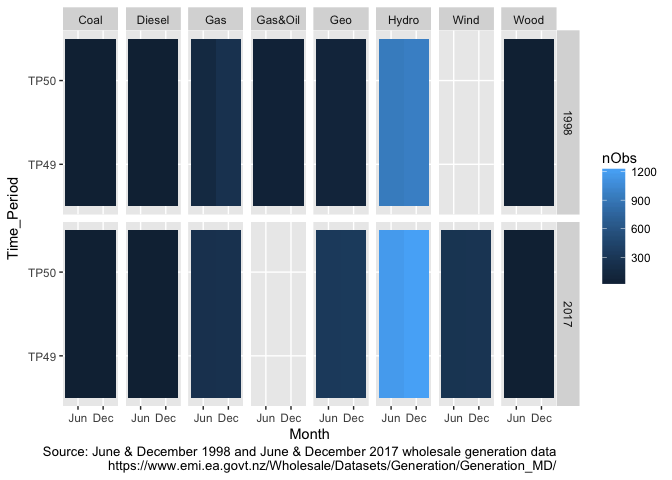
\includegraphics{nzGenerationHistory_files/figure-latex/explore NA-1.pdf}

We therefore remove TP49 \& TP50 from the data for the rest of the
analysis.

\begin{Shaded}
\begin{Highlighting}[]
\NormalTok{cleanDT <-}\StringTok{ }\NormalTok{genDT[}\OperatorTok{!}\KeywordTok{is.na}\NormalTok{(kWh)]}
\NormalTok{cleanDT <-}\StringTok{ }\KeywordTok{droplevels}\NormalTok{(cleanDT)}
\end{Highlighting}
\end{Shaded}

\section{Generation profiles}\label{generation-profiles}

\subsection{Half hourly profiles by
month}\label{half-hourly-profiles-by-month}

This plot replicates one of those found in
\href{https://www.sciencedirect.com/science/article/pii/S0301421516307017\#f0025}{Staffel,
2018} for the UK to show how the different components of generation have
changed over time.

\begin{Shaded}
\begin{Highlighting}[]
\CommentTok{# See how we turned off printing the code into the report}

\CommentTok{# create an aggregated tabe summing generation by fuel, date and time period. This is what data.table is really good at}
\NormalTok{plotDT <-}\StringTok{ }\NormalTok{cleanDT[, }
\NormalTok{                       .(}\DataTypeTok{totalkWh =} \KeywordTok{sum}\NormalTok{(kWh),}
                         \DataTypeTok{nObs =}\NormalTok{ .N),}
\NormalTok{                       keyby =}\StringTok{ }\NormalTok{.(Time_Period, r_month, r_year, Fuel_Code)]}

\CommentTok{# > Use the new data to draw a chart of all generation in the data ----}
\KeywordTok{ggplot}\NormalTok{(plotDT, }
       \KeywordTok{aes}\NormalTok{(}\DataTypeTok{x =}\NormalTok{ Time_Period, }\DataTypeTok{y =}\NormalTok{ totalkWh}\OperatorTok{/}\DecValTok{1000000}\NormalTok{, }\DataTypeTok{fill =}\NormalTok{ Fuel_Code)) }\OperatorTok{+}
\StringTok{  }\KeywordTok{geom_col}\NormalTok{() }\OperatorTok{+}
\StringTok{  }\KeywordTok{facet_grid}\NormalTok{(r_month }\OperatorTok{~}\StringTok{ }\NormalTok{r_year) }\OperatorTok{+}
\StringTok{  }\KeywordTok{labs}\NormalTok{(}\DataTypeTok{caption =}\NormalTok{ ggParams}\OperatorTok{$}\NormalTok{figCaption, }\DataTypeTok{y =} \StringTok{"GWh"}\NormalTok{, }\DataTypeTok{x =} \StringTok{"Half hour"}\NormalTok{) }\OperatorTok{+}
\StringTok{  }\KeywordTok{theme}\NormalTok{(}\DataTypeTok{legend.title=}\KeywordTok{element_blank}\NormalTok{())}
\end{Highlighting}
\end{Shaded}

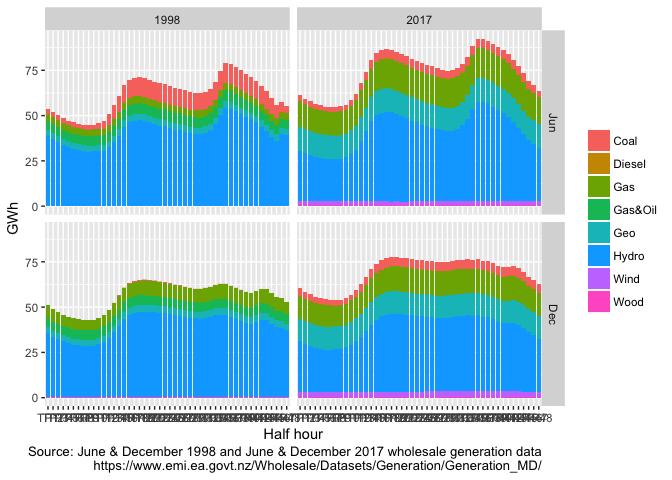
\includegraphics{nzGenerationHistory_files/figure-latex/profile plot by month-1.pdf}

\subsection{Half hourly profiles by day of the
month}\label{half-hourly-profiles-by-day-of-the-month}

This plot shows the profiles for each day of each month joined end to
end.

\begin{quote}
requires creation of true dateTime\ldots{}
\end{quote}

\begin{Shaded}
\begin{Highlighting}[]
\CommentTok{# to do}
\end{Highlighting}
\end{Shaded}

\section{Discuss your results}\label{discuss-your-results}

here

\section{Conclusions}\label{conclusions}

go here

\section{References}\label{references}


\end{document}
